\documentclass[tikz,border=10pt]{standalone}
% No extra TikZ libraries needed.
\begin{document}
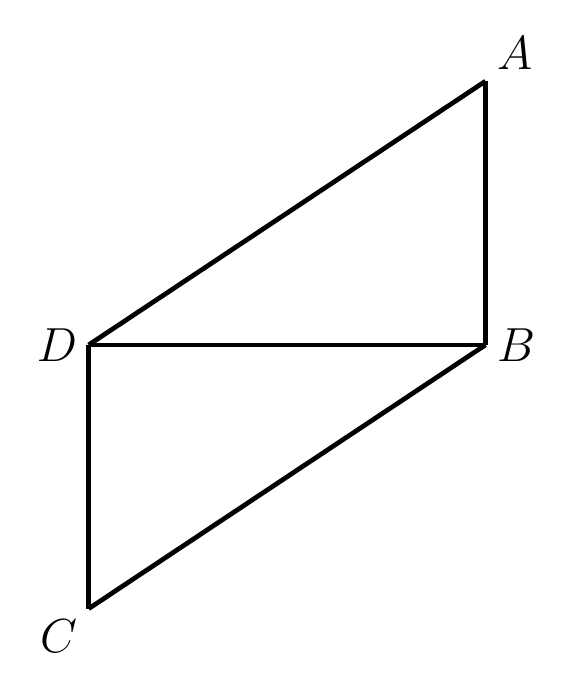
\begin{tikzpicture}[line join=round, line width=1.7pt]
  % Named vertices (pixel -> units: x=(px-188)*0.02139, y=(222.5-py)*0.02139)
  \coordinate (A) at (2.52,3.35);
  \coordinate (B) at (2.52,0);
  \coordinate (C) at (-2.52,-3.35);
  \coordinate (D) at (-2.52,0);

  % Solid segments: A-B, B-D, D-C, A-D, B-C
  \draw (A) -- (B);
  \draw (B) -- (D);
  \draw (D) -- (C);
  \draw (A) -- (D);
  \draw (B) -- (C);

  % Labels placed outside the figure
  \node[above right, font=\fontsize{17.5}{21}\selectfont] at (A) {$A$};
  \node[right, font=\fontsize{17.5}{21}\selectfont] at (B) {$B$};
  \node[below left, font=\fontsize{17.5}{21}\selectfont] at (C) {$C$};
  \node[left, font=\fontsize{17.5}{21}\selectfont] at (D) {$D$};
\end{tikzpicture}
\end{document}